Las \textbf{Estructuras (\textit{Structures})} son objetos estáticos que forman parte del entorno del juego, como edificios,
árboles o rocas. Al ser colocados, su posición, rotación y escala pueden editarse mediante \textit{Gizmos} o a través
de su panel de configuración. Cada estructura permite configurar sus colisionadores (\textit{Colliders}), que definen
las interacciones físicas con el jugador y otros elementos del juego. Actualmente se soportan dos tipos de colisionador:
cubo (\textit{Cube}), de uso general, y rampa (\textit{Slope}), un colisionador de forma piramidal diseñado para
superficies inclinadas que permiten al jugador desplazarse hacia zonas de mayor altura. Adicionalmente, cualquier
estructura puede configurarse como tienda (\textit{Shop}), habilitando la compra de ítems por parte de los jugadores.

\begin{figure}[H]
    \centering
    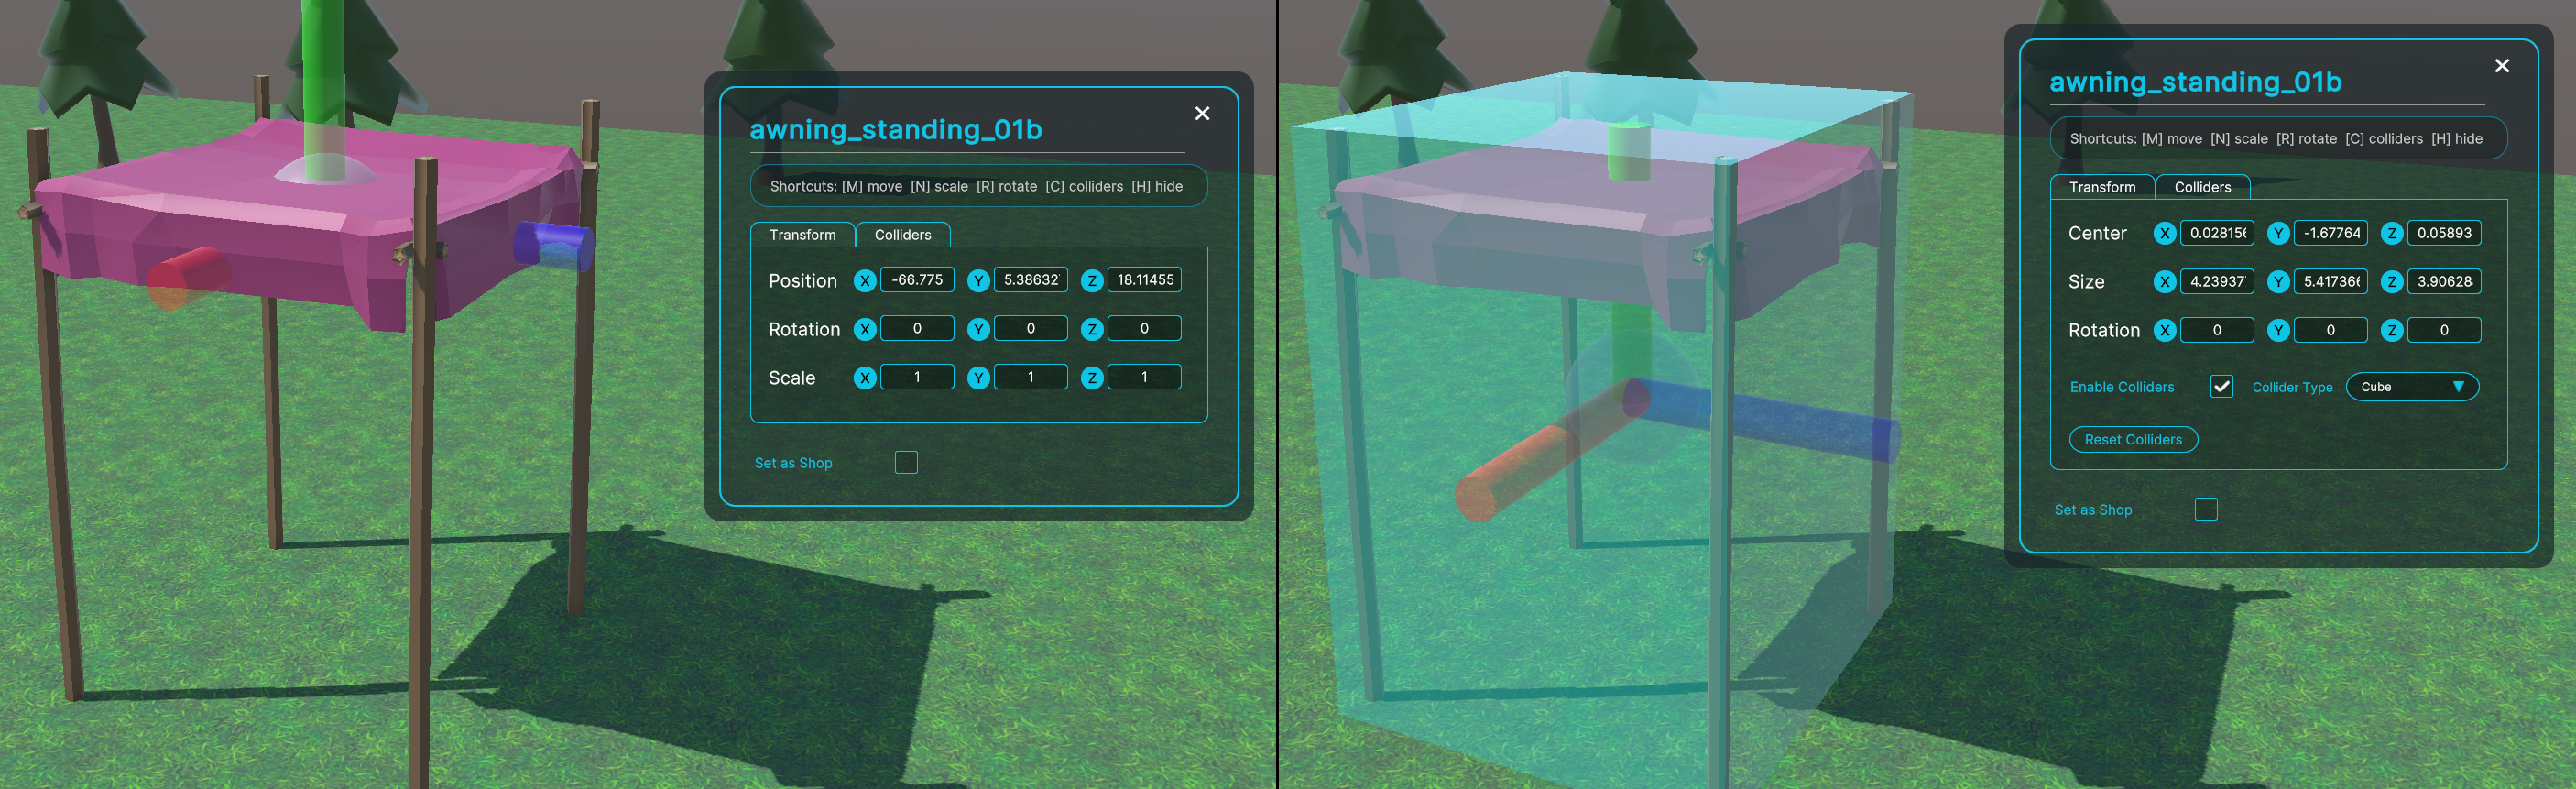
\includegraphics[width=\textwidth]{img/08-implemented-solution/world-editor/structure.jpg}
    \caption{Estructura seleccionada donde se puede ver tambien las pestañas de transformacion y colisionadores.}
\end{figure}

\begin{figure}[H]
    \centering
    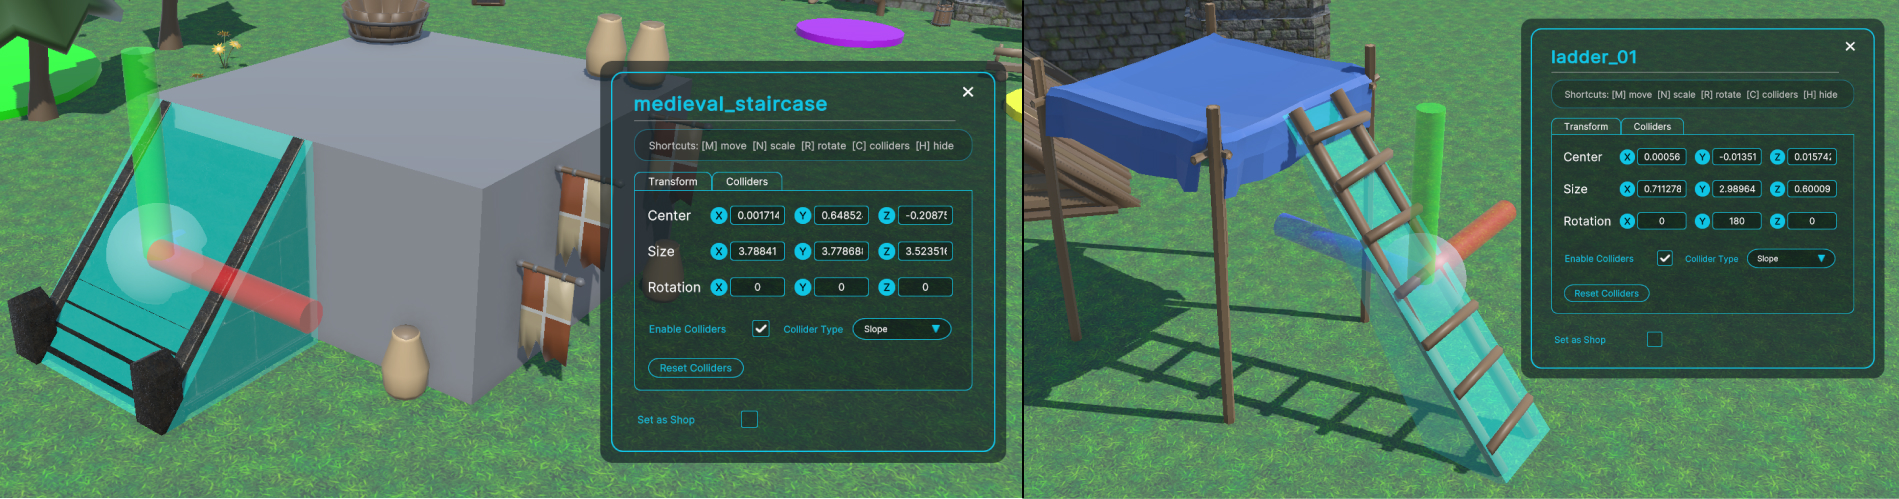
\includegraphics[width=\textwidth]{img/08-implemented-solution/world-editor/slope-collider.jpg}
    \caption{Estructuras con colisionador de tipo rampa con transformaciones aplicadas.}
\end{figure}

\begin{figure}[H]
    \centering
    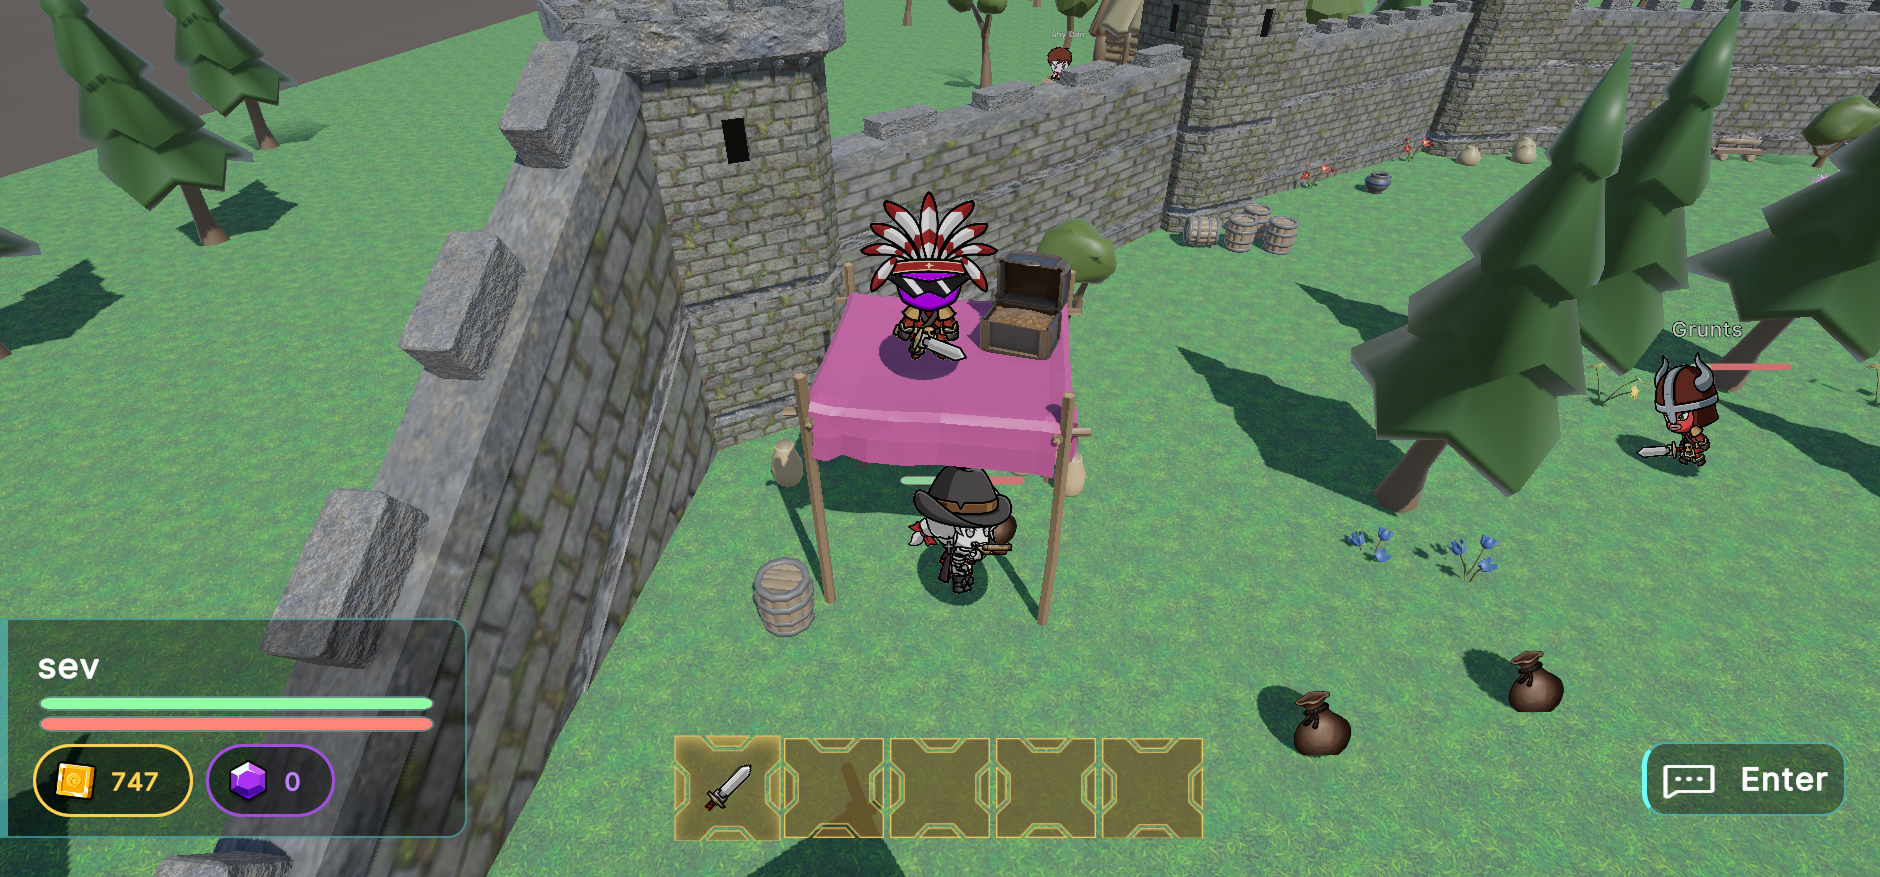
\includegraphics[width=\textwidth]{img/08-implemented-solution/product/player-on-structure.jpg}
    \caption{Captura de un jugador sobre una carpa con los collisionadores modificados}
\end{figure}

\subsubsection{Estructuras Predeterminado y Personalizado}

Al iniciar el editor de mundos por primera vez, el creador no tiene estructuras disponibles para colocar, 
por lo que el editor ofrece una biblioteca de modelos predeterminados que los creadores pueden descargar libremente mediante la seccion de \textit{Default Content}.
Estos modelos predeterminados ofrecen una variedad de opciones para enriquecer la ambientación y composición visual de las zonas.

\vspace{0.25cm}

Además de utilizar modelos predeterminados, el creador tiene la opción de importar sus propios modelos 3D 
personalizados mediante el \textit{Custom Model Importer}. Esto le permite diseñar y emplear sus propios \textit{assets} visuales, incorporando contenido 
único y personalizado en sus mundos.

\begin{figure}[H]
    \centering
    
\includegraphics[width=\textwidth]{img/08-implemented-solution/world-editor/import-model.jpg}
    \caption{Modelo importado en la escena.}
\end{figure}

\subsubsection{Atributos de Calidad}
Un aspecto fundamental del editor es su enfoque en la usabilidad, con una interfaz intuitiva y accesible que permite a los 
creadores de mundos diseñar experiencias complejas sin necesidad de conocimientos técnicos avanzados. 
Se implementaron paneles de configuración claros y herramientas de edición visual que facilitan la colocación y 
personalización de objetos, así como la gestión de recursos y la publicación de mundos.

\paragraph{Gizmos}
Para mejorar la experiencia de edición, se implementaron \textit{Gizmos} personalizados 
que permiten a los creadores manipular visualmente la posición, rotación y escala de los objetos colocados en la escena.

  \begin{figure}[H]
  \centering
  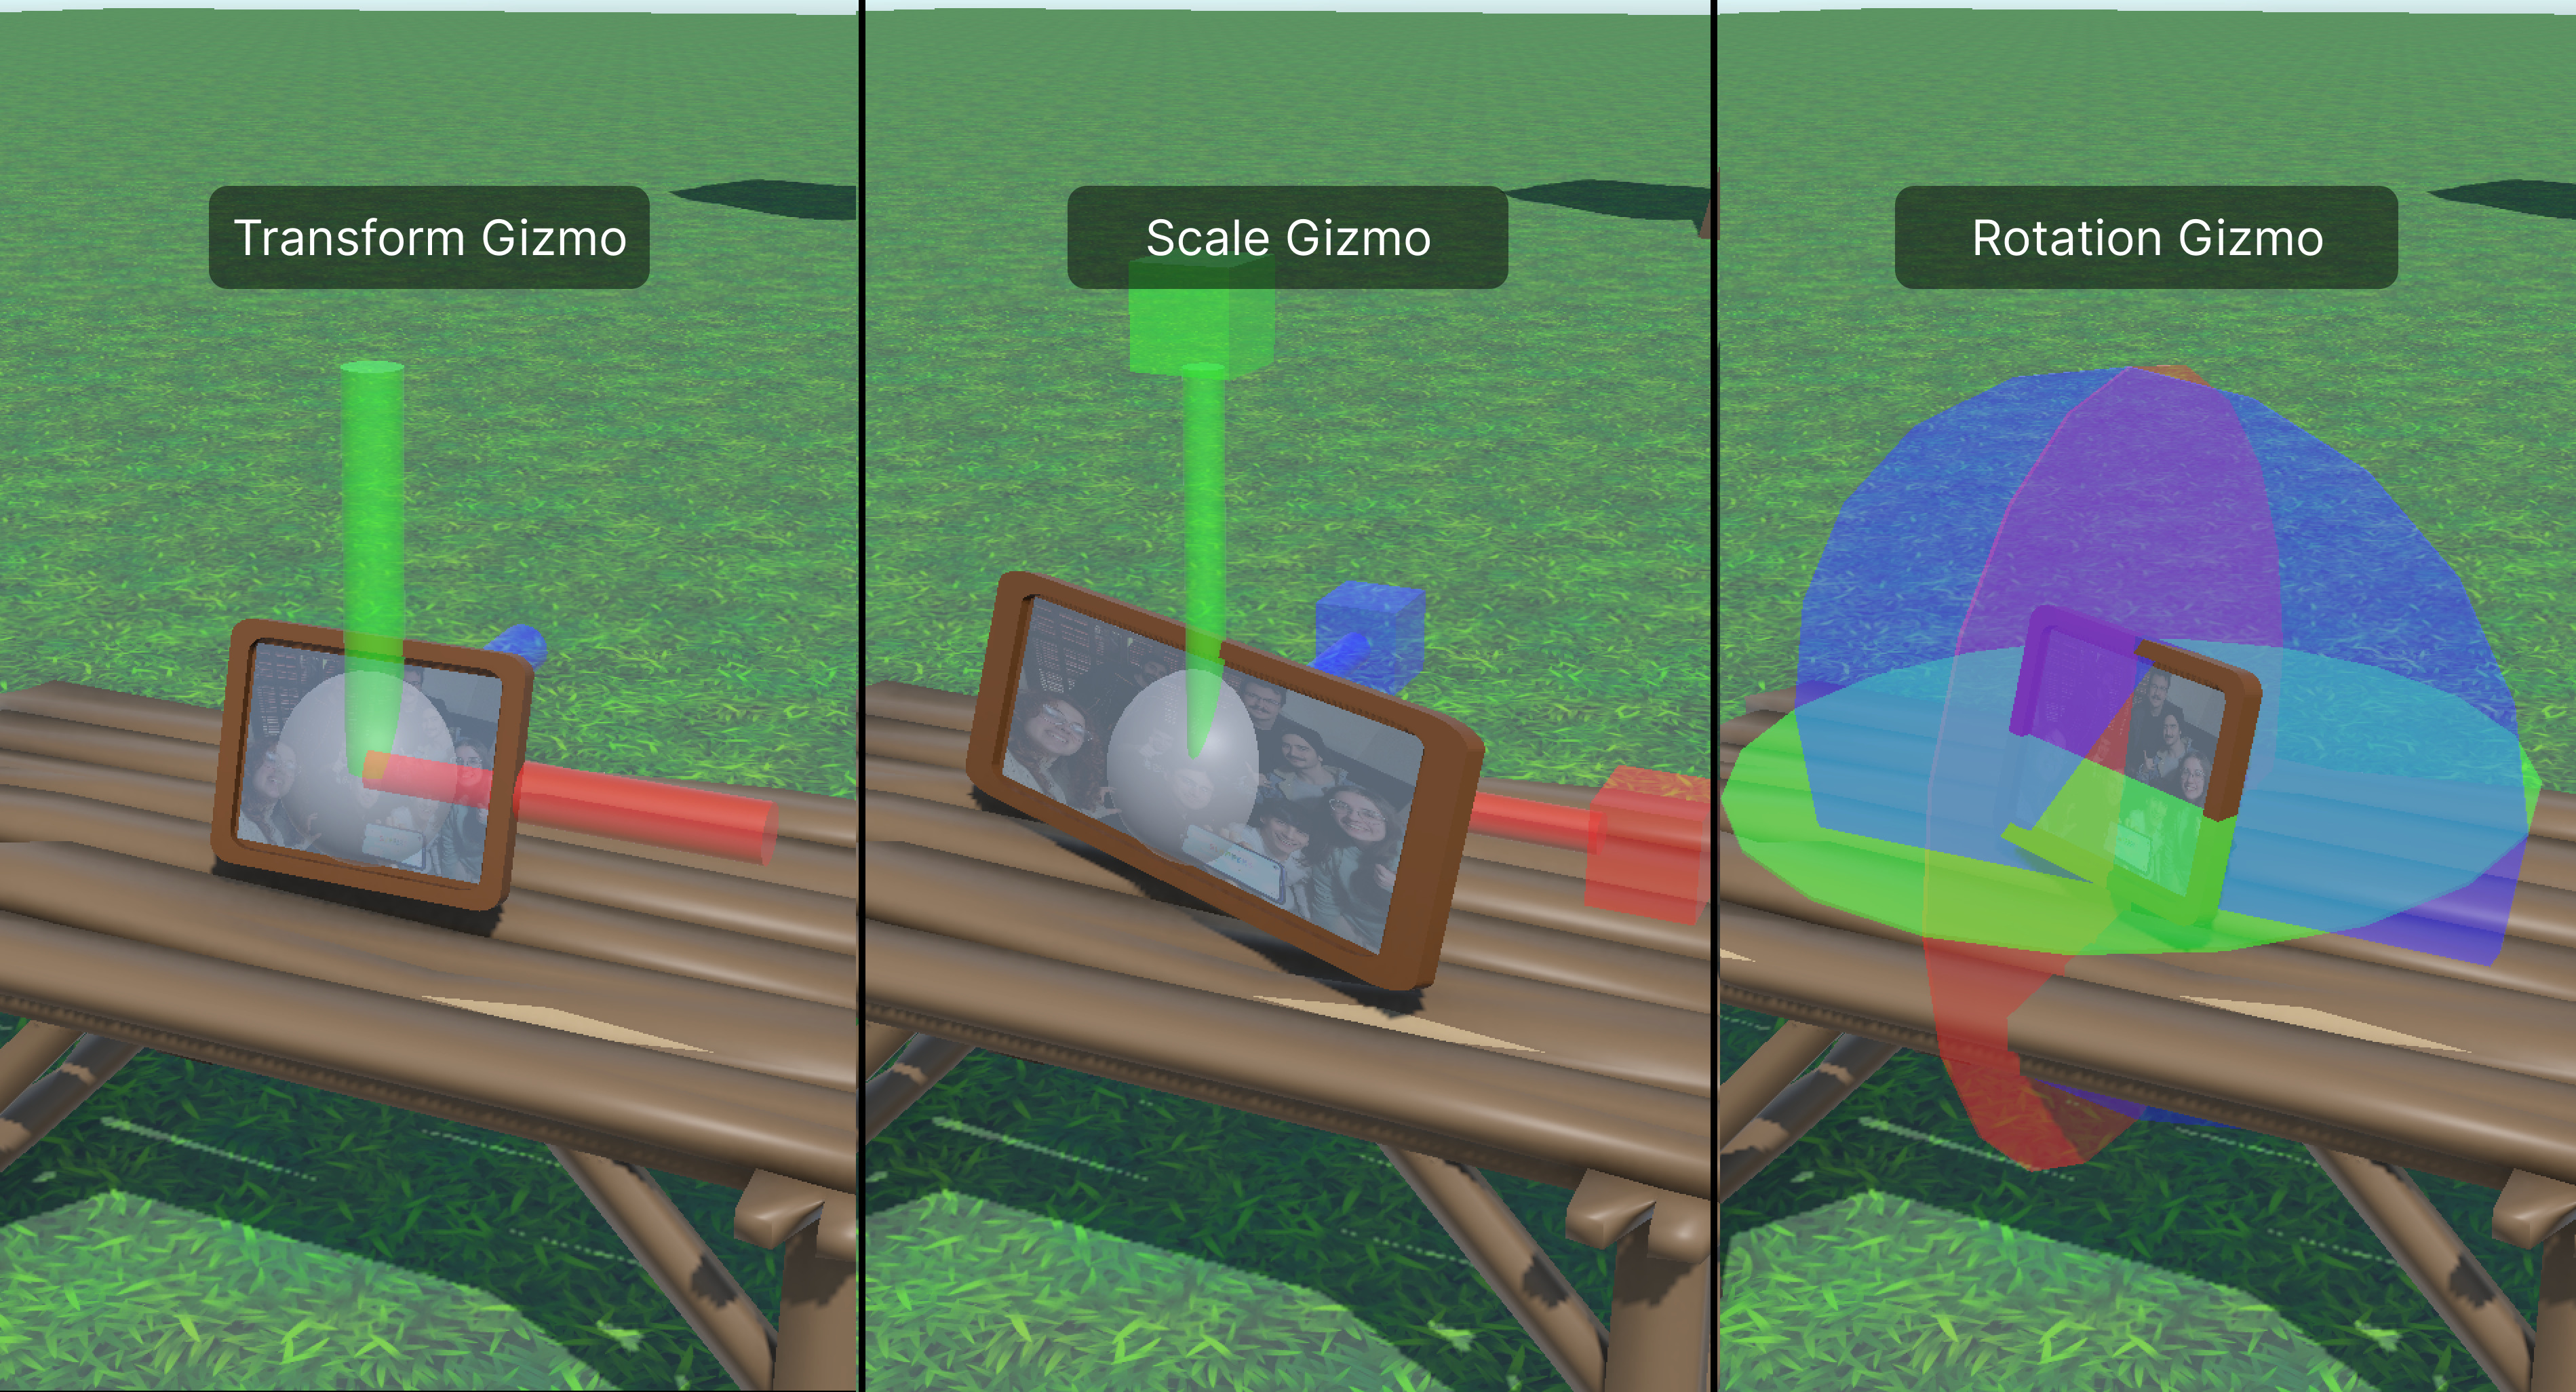
\includegraphics[width=\textwidth]{img/08-implemented-solution/world-editor/gizmos.jpg}
  \caption{Gizmos implementados.}
  \label{fig:gizmos}
\end{figure}

\paragraph{Editor de Models 3D}
La importación de modelos 3D desde internet puede introducir problemas de escala o rotación, ya que el formato \texttt{.glb} 
no define una convención de orientación, lo que con frecuencia produce modelos importados con resultados no deseables. 
Para resolver esto, se incorporó un editor de modelos 3D, que permite a los  creadores ajustar visualmente la escala
y la rotación antes de finalizar la importación al mundo, garantizando que el 
modelo se integre correctamente en la escena sin necesidad de herramientas externas. El editor también permite 
definir si el modelo tendrá o no colisiones al colocarse, lo que resulta útil para elementos decorativos que no 
requieren colisionadores y mejora la experiencia al ubicar múltiples modelos sin tener que configurar cada 
uno de forma individual luego de su colocación. El editor de modelos también cuenta con una pestaña 
dedicada a configurar qué modelo de cofre se utiliza por defecto al colocar uno.

\begin{figure}[H]
\centering

\includegraphics[width=\textwidth]{img/08-implemented-solution/world-editor/model-editor.jpg}
\caption{Editor de modelos 3D.}
\label{fig:model-editor}
\end{figure}